\documentclass{book}

\usepackage{amsmath}
\usepackage{graphicx}
\usepackage{subcaption}
\usepackage{setspace}
\usepackage{titlepic}

\graphicspath{ {images/} }

\title{This is a title}
\author{This is an author}
\titlepic{
\includegraphics[width=5cm]{polimi}}
\date{\vspace{-5ex}}

%\setcounter{tocdepth}{1} % Show sections.
%\setcounter{tocdepth}{2} % + subsections.
\setcounter{tocdepth}{3} % + subsubsections.
%\setcounter{tocdepth}{4} % + paragraphs.
%\setcounter{tocdepth}{5} % + subparagraphs.

\begin{document}

\pagenumbering{gobble}

\maketitle

\pagenumbering{roman}

\cleardoublepage
\newpage

\doublespacing % Double the spacing for the ToC.
\tableofcontents
\singlespacing % Reset the spacing.

\cleardoublepage
\newpage

\listoffigures

\cleardoublepage
\newpage

\listoftables

\cleardoublepage
\newpage

\pagenumbering{arabic}

\section{Introduction}

This is a section.

\subsection{Subsection}

This is a subsection.

\paragraph{Paragraph} 

This is a paragraph in a subsection.

\subparagraph{Subparagraph} 
 
This is a subparagraph in a subsection.

\section{Math}

This section contains an equation:

\begin{equation}
f(x) = x^2 + 2
\end{equation}

If you don't want your equation to be numbered, use *:

\begin{equation*}
f(x) = x^2 + 2
\end{equation*}

Moreover, equations can be aligned:

\begin{align*}
f(x) &= x^2\\
g(x) &= \frac{1}{x}\\
g(x) &= \frac{1}{\sqrt{x}} \\
F(x) &= \int^a_b \frac{1}{3}x^3
\end{align*}

I can also have math embedded in a text delimited by the \$ sign, like this: $f(x) = x^2 + 2$ .

\paragraph{} 

Finally, we have a matrix:

\begin{equation*}
\left[
\begin{matrix}
1 & 0\\
0 & 1
\end{matrix}
\right]
\end{equation*}

The left and right notation is used to scale the brackets, but can also be used with other elements. 

\section{Figures}

\begin{figure}
  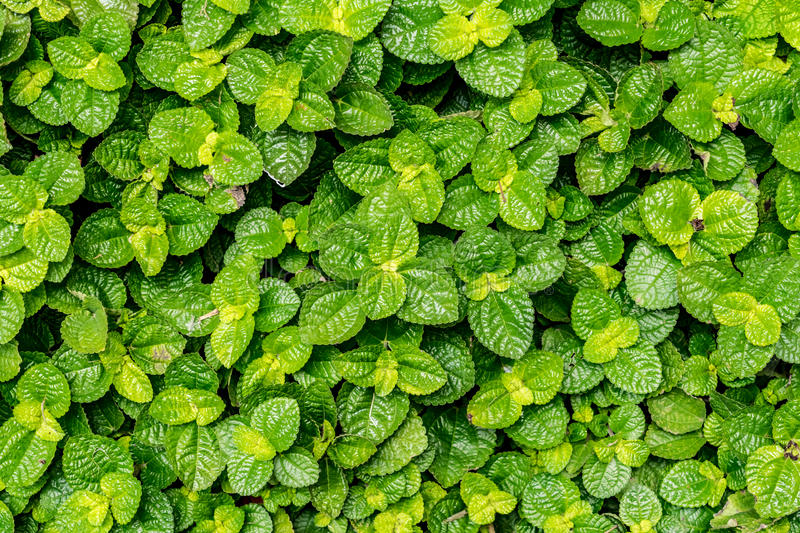
\includegraphics[width=\linewidth]{mint.jpg}
  \caption{Some mint.}
  \label{fig:mint1}
\end{figure}

Figure \ref{fig:mint1} shows some mint.

\begin{figure}[h!]
  \centering
  \begin{subfigure}[b]{0.4\linewidth}
    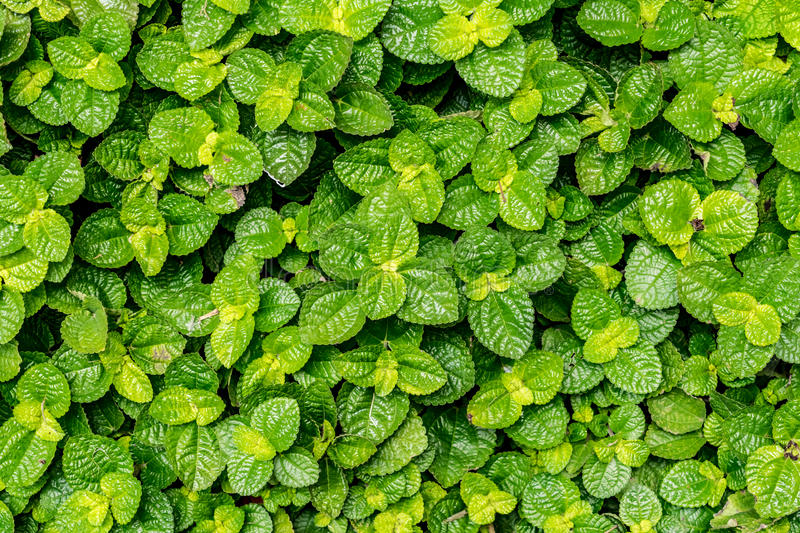
\includegraphics[width=\linewidth]{mint.jpg}
    \caption{Mint.}
  \end{subfigure}
  \begin{subfigure}[b]{0.4\linewidth}
    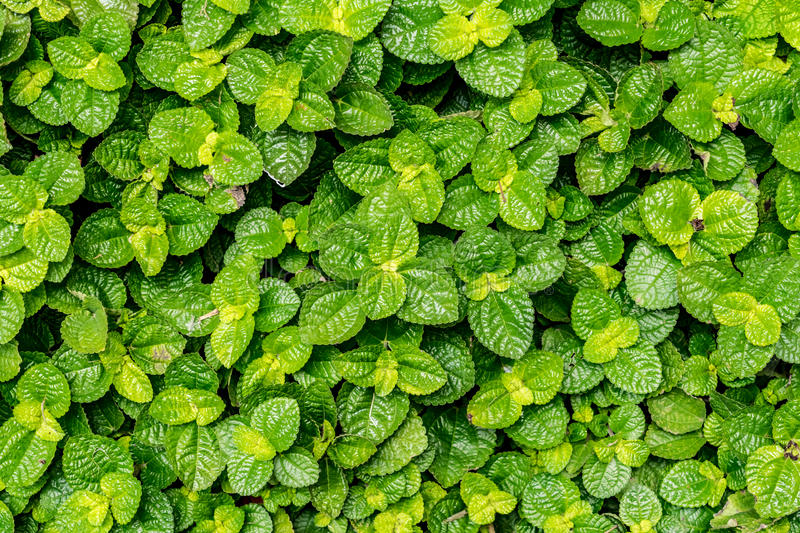
\includegraphics[width=\linewidth]{mint.jpg}
    \caption{More mint.}
  \end{subfigure}
  \caption{The same mint. Twice.}
  \label{fig:mints1}
\end{figure}

\paragraph{} 

Figure \ref{fig:mints1} shows even more mint. Here I have set linewidth to .4 instead of 0.5 ($0.5 * 2 = 1$), since you always have to set it .1 less than you expect.

\begin{figure}[h!]
  \centering
  \begin{subfigure}[b]{0.2\linewidth}
    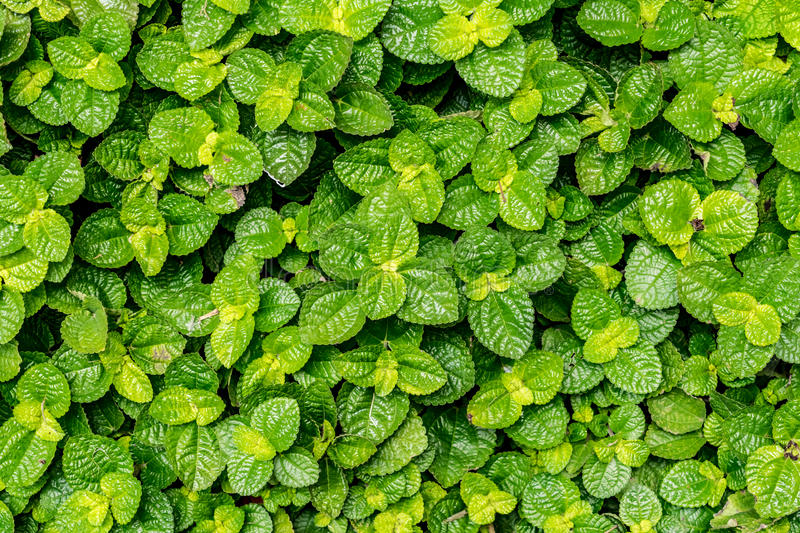
\includegraphics[width=\linewidth]{mint.jpg}
     \caption{Mint.}
  \end{subfigure}
  \begin{subfigure}[b]{0.2\linewidth}
    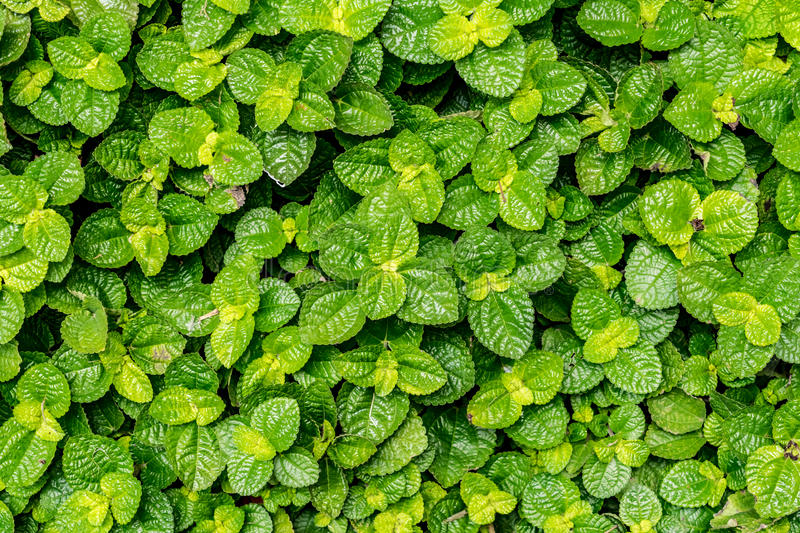
\includegraphics[width=\linewidth]{mint.jpg}
    \caption{More mint.}
  \end{subfigure}
  \begin{subfigure}[b]{0.2\linewidth}
    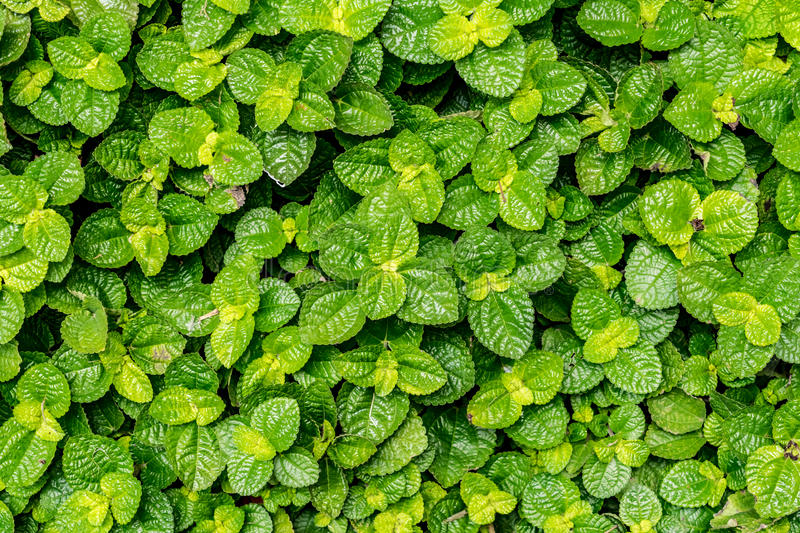
\includegraphics[width=\linewidth]{mint.jpg}
    \caption{Fresh mint.}
  \end{subfigure}
  \begin{subfigure}[b]{0.5\linewidth}
    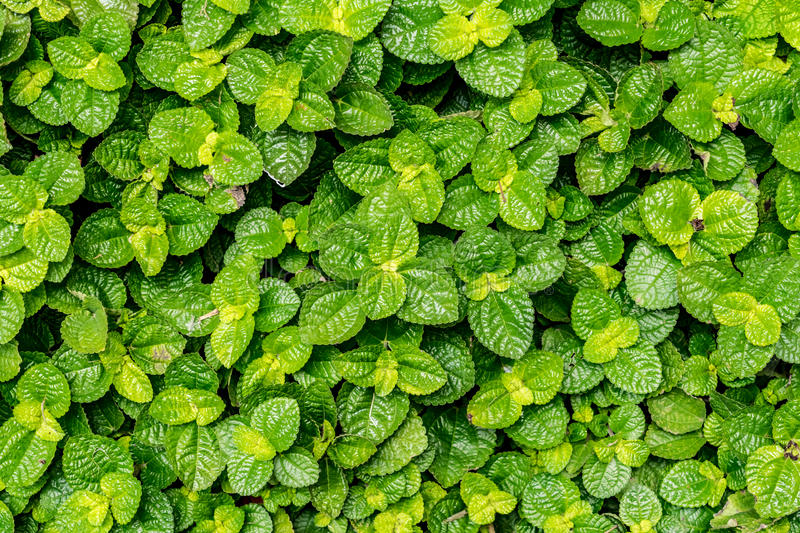
\includegraphics[width=\linewidth]{mint.jpg}
    \caption{Too much mint.}
  \end{subfigure}
  \caption{The same mint. Multiple times. Fresh as ever.}
  \label{fig:mints2}
\end{figure}

\paragraph{} 

Figure \ref{fig:mints1} shows a lot of mint on multiple rows.

\addtocontents{toc}{\setcounter{tocdepth}{1}} % Set depth to 1.
\section{Section which subsections and subsubsections I want to hide in the ToC}

This is a section.

\subsection{Hidden subsection in the ToC}

This is a subsection.

\subsection{Hidden subsubsection in the ToC}

This is a subsubsection.

\addtocontents{toc}{\setcounter{tocdepth}{3}} % Reset the depth to default.
\section{Section which subsections and subsubsections I want to show in the ToC}

This is a section.

\subsection{Visible subsection in the ToC}

This is a subsection.

\subsection{Visible subsubsection in the ToC}

This is a subsubsection.

\section{Citations and footnotes section}

This is a random citation \cite{DUMMY:1} embeddeed in text.

\paragraph{}

This is some example text\footnote{\label{myfootnote}Hello footnote}.

\paragraph{}

I'm referring to footnote \ref{myfootnote}.

\newpage
\cleardoublepage

\bibliography{bibliography/bibliography} 
\bibliographystyle{ieeetr}

\end{document}